\section{LOG2 Base-2 Logarithm Function}

\subsection{Usage}

Computes the \verb|log2| function for its argument.  The general
syntax for its use is
\begin{verbatim}
  y = log2(x)
\end{verbatim}
where \verb|x| is an \verb|n|-dimensional array of numerical type.
Integer types are promoted to the \verb|double| type prior to
calculation of the \verb|log2| function.  Output \verb|y| is of the
same size as the input \verb|x|. For strictly positive, real inputs, 
the output type is the same as the input.
For negative and complex arguments, the output is complex.
\subsection{Example}

The following piece of code plots the real-valued \verb|log2|
function over the interval \verb|[1,100]|:
\begin{verbatim}
--> x = linspace(1,100);
--> plot(x,log2(x))
--> xlabel('x');
--> ylabel('log2(x)');
\end{verbatim}


\centerline{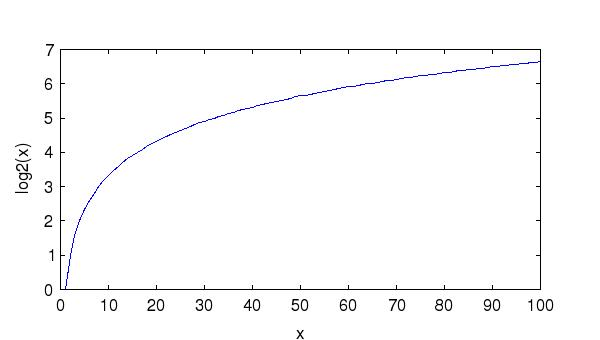
\includegraphics[width=8cm]{log2plot}}

